\documentclass{article}
\usepackage[UTF8]{ctex}
\usepackage{graphicx}		%插入图片
\usepackage{indentfirst}	%首行缩进
\usepackage{float}			%浮动体
\usepackage{amsmath}		%矩阵

\setlength{\parindent}{2em}	%首行缩进2汉字

\usepackage{graphicx} %插入图片的宏包
\usepackage{float} %设置图片浮动位置的宏包
\usepackage{subfigure} %插入多图时用子图显示的宏包

\begin{document}

\title{第12组数据故事创作}
\maketitle						%生成标题


琼瑶是一位在中国文学史上留下深刻印记的知名作家,她的小说作品不仅情感丰富,而且字数众多,完稿时间与出版时间也各具特色。下面,我们将通过琼瑶小说作品的字数-完稿时间分布图和完稿到出版的时间差分布图,来讲述一个关于她的数据故事。

\section{字数-完稿时间分布图}

下图是琼瑶小说作品的字数-完稿时间分布图。

从图中我们可以看到,琼瑶的小说创作历程跨越了多个年份,从1963年的《窗外》开始,一直延续到2010年代。这部《窗外》以162400字的篇幅,拉开了琼瑶小说创作的序幕。随后,她的作品如雨后春笋般涌现,每一部都承载着独特的情感和故事。

在1970年代,琼瑶的小说字数大多在100000至160000字之间,如《水灵》、《浪花》和《海鸥飞处》等作品。这些小说以细腻的情感描绘和曲折的故事情节,赢得了广大读者的喜爱。随着年代的推移,琼瑶的小说字数也逐渐增加,反映了她在文学创作上的不断探索和成长。

进入1980年代,琼瑶的小说字数普遍超过了100000字,部分作品甚至达到了近200000字的篇幅。这一时期的作品,不仅在字数上有所增加,更在情感和故事的深度上达到了新的高度。

到了1990年代,琼瑶的小说创作迎来了巅峰期。《还珠格格第一部》以243500字的篇幅,成为了她这一时期的代表作之一。随后,《苍天有泪》和《还珠格格第二部》更是分别以305900字和583200字的惊人篇幅,创造了琼瑶小说字数的新高。这些作品不仅字数庞大,更在情节设计、人物塑造和情感表达上达到了炉火纯青的地步。

然而,进入21世纪之后,琼瑶减少了文学小说的创作,而把心思更多放在了《还珠格格》系列的打造,以及相应的影视化工作。可以看到,相比其早年,琼瑶在晚年写作速度上有所减缓,但是其作品的长度却急剧增长。这可能受到她的年龄、创作风格转变、市场环境等因素影响。

从这张字数-完稿时间分布图中,我们还可以发现一些有趣的规律。例如,琼瑶早期的文学小说创作在字数方面往往呈现出一种“波浪式”的增长趋势,即在某个时期字数会有所增加,而在下一个时期则可能会略有减少。这种变化可能与她的创作灵感、生活经历以及市场环境等多种因素有关,我们可能可以结合其生平给出进一步分析。
\begin{figure}[H] %H为当前位置,!htb为忽略美学标准,htbp为浮动图形
\centering %图片居中
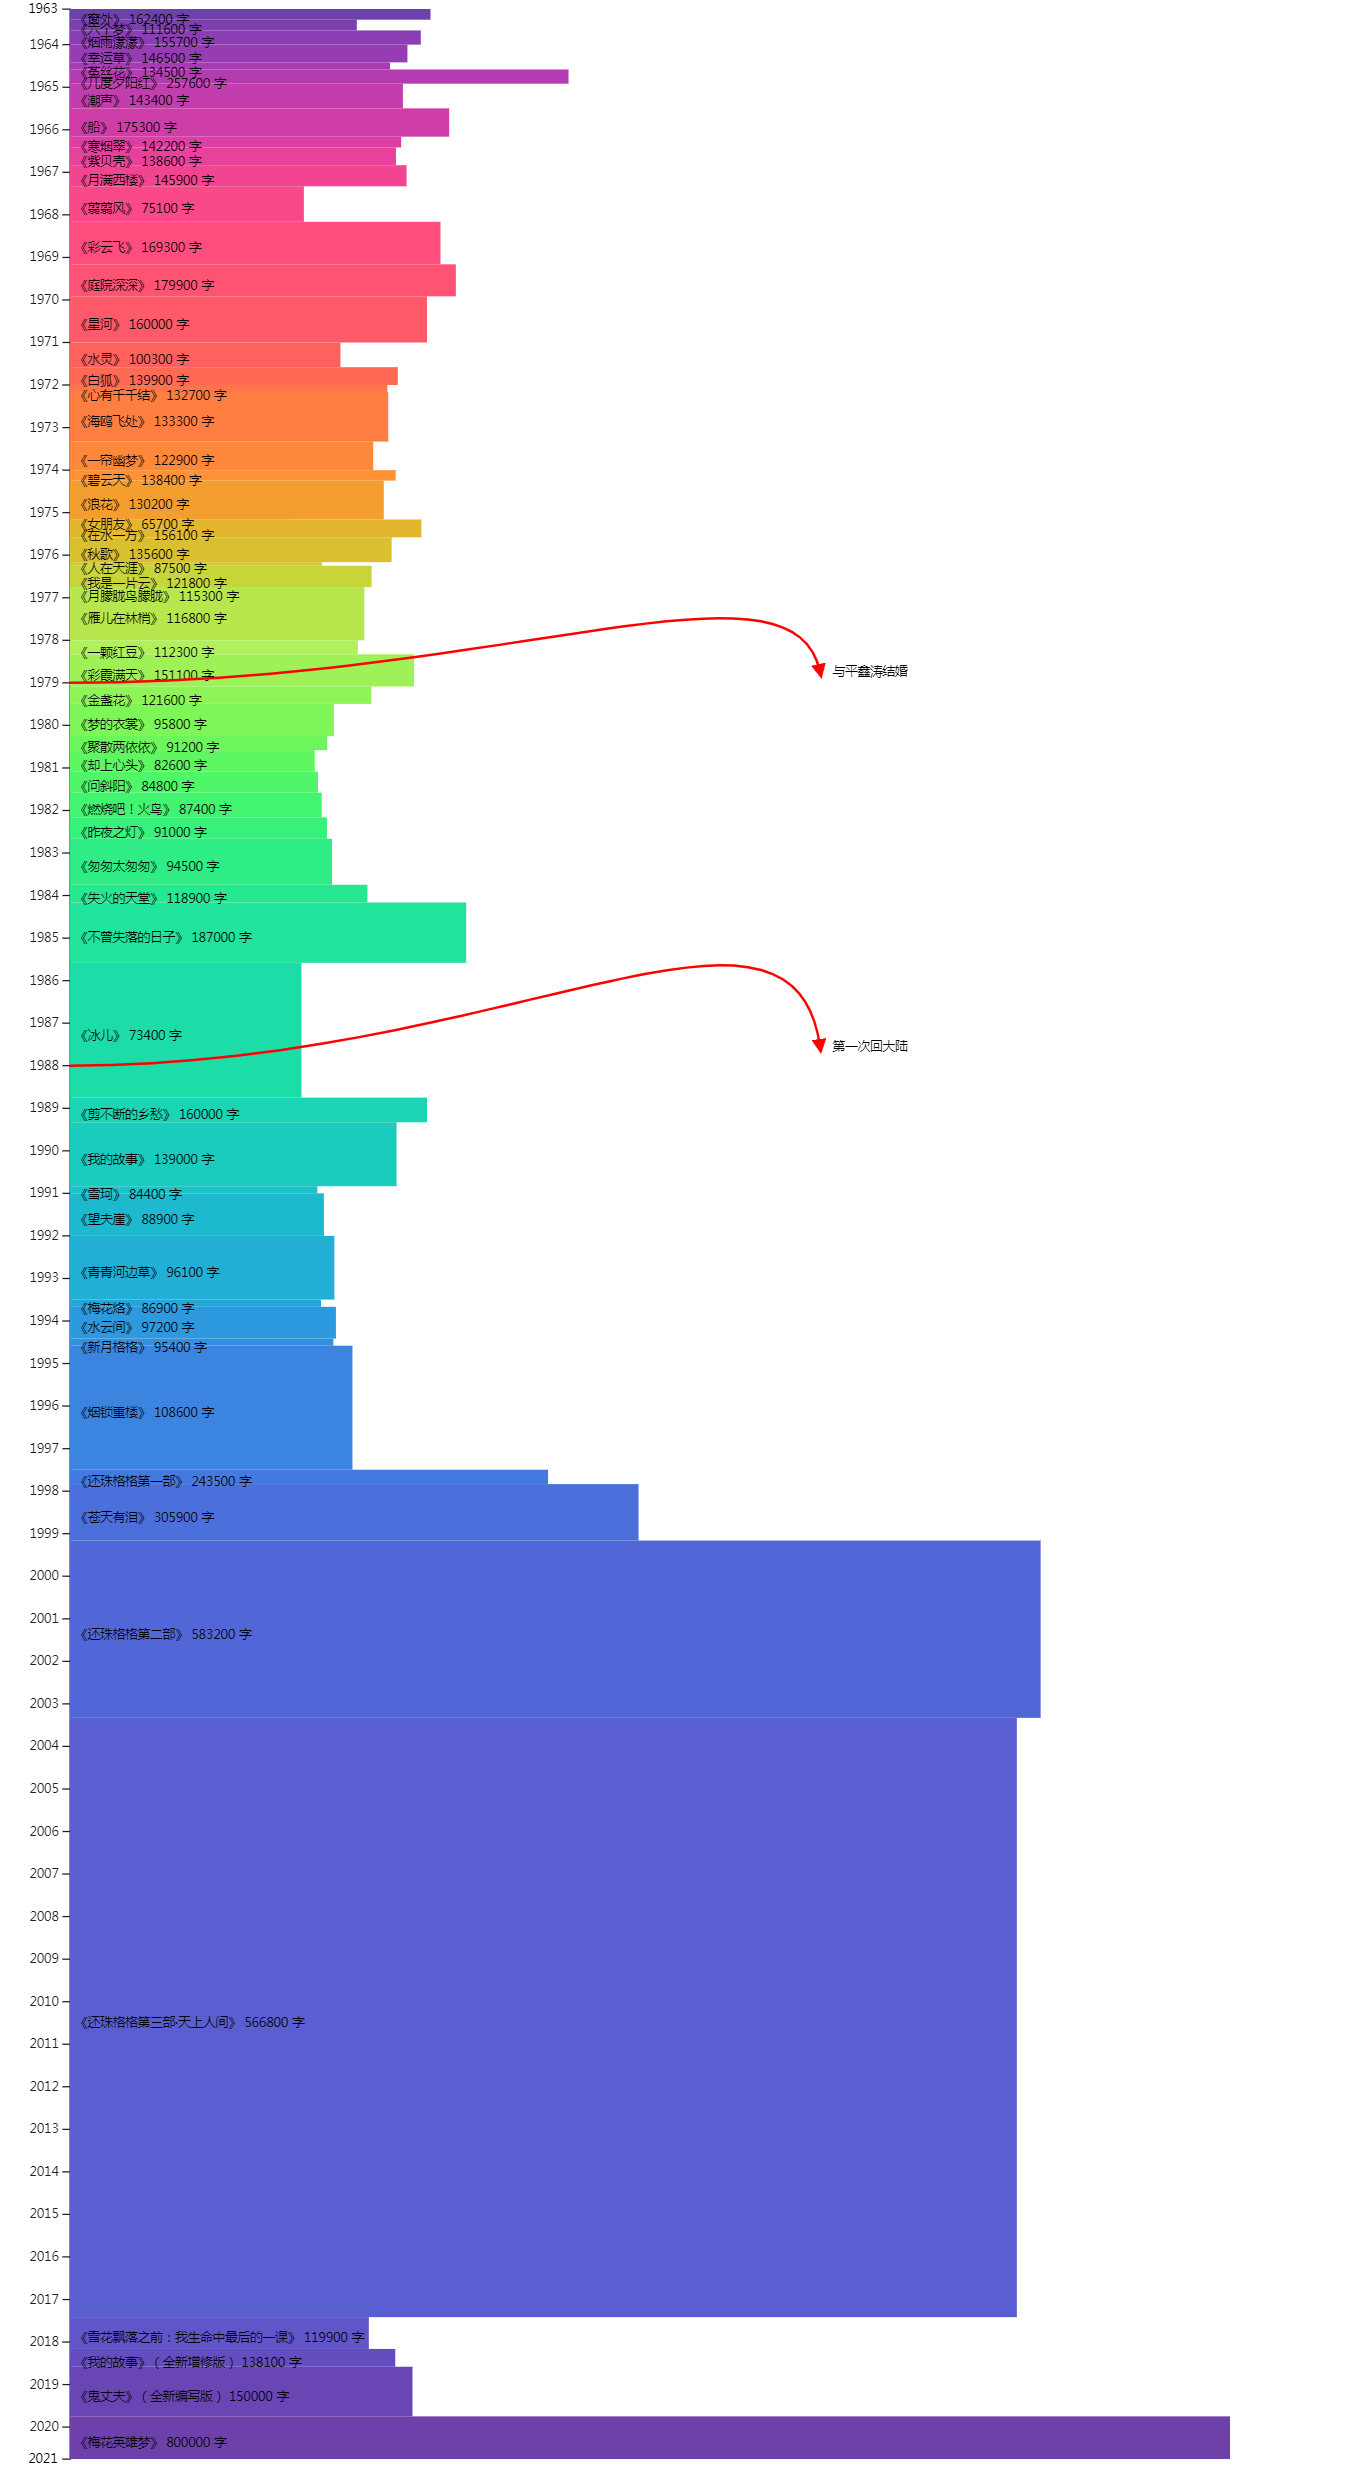
\includegraphics[width=0.7\textwidth]{pic/pic1} %插入图片,[]中设置图片大小,{}中是图片文件名
\caption{琼瑶小说字数-完稿时间分布图} %最终文档中希望显示的图片标题
\label{Fig.p1} %用于文内引用的标签
\end{figure}

\section{完稿到出版的时间差分布图}

下图是琼瑶小说作品的完稿到出版的时间差分布图,总的来说,琼瑶的大多数作品都能在一年以内与读者见面。

首先,我们关注的是琼瑶与平鑫涛结婚前的时期。在这一阶段,琼瑶的作品完稿到出版的时间差分布较为分散,有的作品能够迅速面世,而有的则需要等待数百天之久。这可能与当时的出版环境、市场需求以及琼瑶个人的创作节奏有关。但无论如何,这些作品都以其独特的魅力和情感深度,赢得了读者的广泛好评。

接下来,我们进入琼瑶与平鑫涛结婚后第一次回大陆前的时期。在这一阶段,琼瑶的作品完稿到出版的时间差相较于上个时间段减小了,大多数作品都能在较短的时间内与读者见面。这可能与琼瑶与平鑫涛的合作更加紧密,以及出版社对琼瑶作品的重视和高效运作有关。这一时期,琼瑶的小说创作达到了巅峰状态,多部经典之作相继问世,如《窗外》、《几度夕阳红》等,深受读者喜爱。

最后,我们关注的是琼瑶第一次回大陆后的时期。在这一阶段,琼瑶的作品完稿到出版的时间差相较于上个时间段没有太大改变。这可能与琼瑶对大陆市场的了解和重视,以及出版社在大陆地区的推广和运作有关。这一时期,琼瑶的小说在大陆地区也取得了巨大的成功,成为了一代读者的共同记忆。
\begin{figure}[H] %H为当前位置,!htb为忽略美学标准,htbp为浮动图形
\centering %图片居中
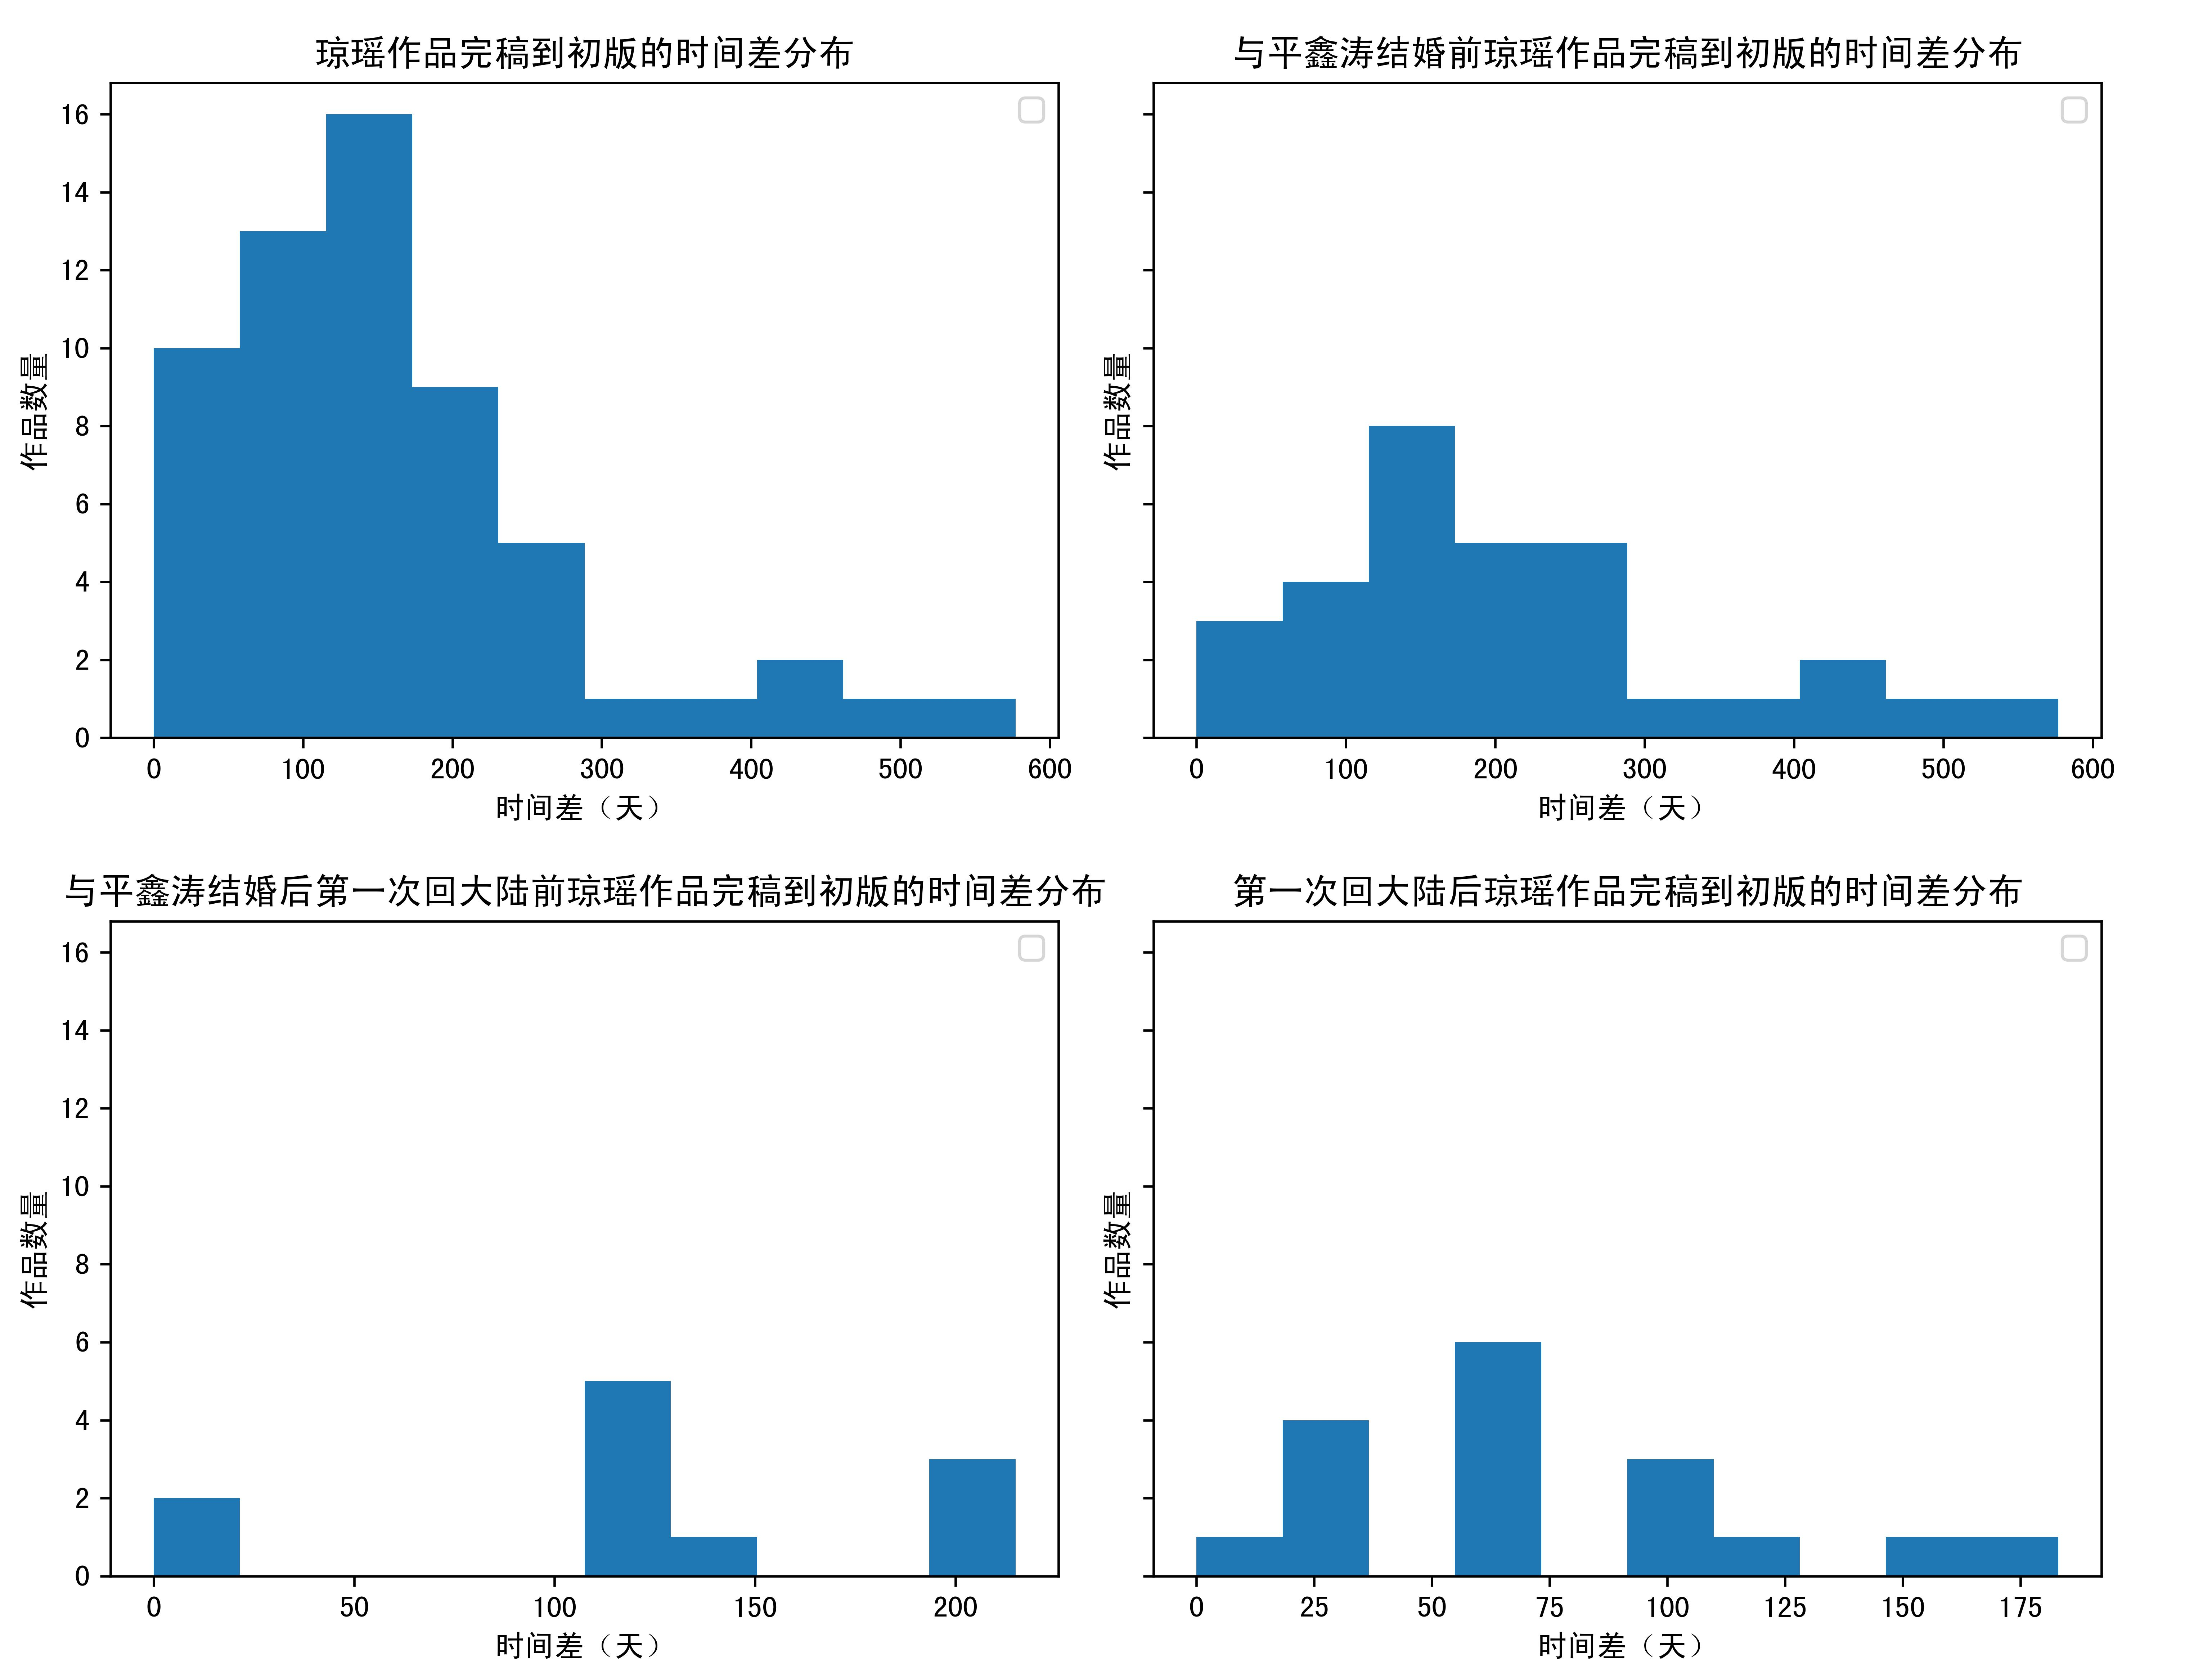
\includegraphics[width=0.7\textwidth]{pic/pic2} %插入图片,[]中设置图片大小,{}中是图片文件名
\caption{琼瑶小说完稿到出版的时间差分布图} %最终文档中希望显示的图片标题
\label{Fig.p2} %用于文内引用的标签
\end{figure}

\end{document}